\documentclass[document.tex]{subfiles}
\begin{document}

\chapter{Algorytm Viterbiego}
\section{Opis działania i zastosowania}
\indent Alogorytm Viterbiego został stworzony i przeanalizowany przez A.J. Viterbiego w 1967r. Jego zadaniem było dekodowanie kodów splotowych. Później odkryto że posiada cechy programowania dynamicznego i wykorzystuje maksymalne prawdopodobieństwo do określenia optymalnego zestawu tranzycji pomiędzy stanami. Algorytm został oryginalnie opracowany z myślą o zastosowaniach w telekomunikacji, ale znalazł zastosowanie w innych dziedzinach, m.in. w przetwarzanie obrazów, lokalizacji i rozpoznawaniu obiektów.\cite{viterbi_tutorial}
\\
\indent Główne zastosowanie algorytmu Viterbiego polega na
dekodowaniu informacji zakodowanych przy pomocy kodów splotowych. Sekwencja kodowana $m = m_1, m_2,...,m_n$, gdzie 
$m_i$ reprezentuje pojedynczy bit informacji, a indeks oznacza kolejność przesyłania. Enkoder splotowy przekształca informację wejściową w zakodowaną sekwencję $U = G(m)$.
Wykorzystuje do tego rejestr przesuwający, sumatory modulo-2 oraz wielomiany generujące(\textit{generator polynomials}) określające związek sumatorów z rejestrem.\cite{Comm_Sklar}\cite{viterbi_tutorial}

\begin{figure}[h]
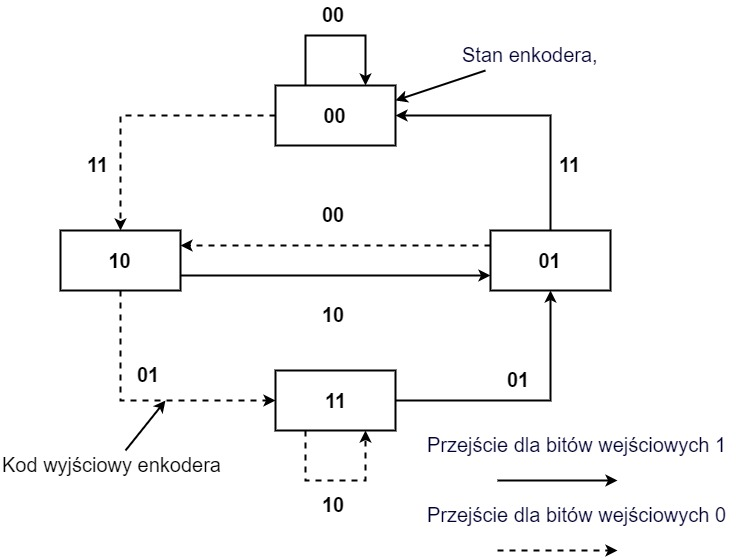
\includegraphics[scale=0.45]{conv_encoder}
\caption{Diagram stanów, dla enkodera o 3 bitowym rejestrze przesuwnym 
i dwóch sumatorach modulo-2 z wielomianami $g_1 = 111, g_2 = 101$ \protect\cite{Comm_Sklar}}
\label{fig:encoder}
\end{figure}
\clearpage
\indent Enkoder splotowy należy do klasy urządzeń zwanych automatami skończonymi(\textit{finite-state machines}), które zachowują informację o poprzednich sygnałach.
Jego działanie można zaprezentować w postaci diagramu stanów(\textit{state diagram}). Bieżący stan reprezentują pierwsze $K - 1$ bity rejestru o pojemności K, a przejścia pomiędzy stanami są określane przez kody wyjściowe.
Dla enkodera z 3 bitowym rejestrem przesuwającym i 2 bitowym wyjściem, stany są określone jako kolejno
$00, 01, 10, 11$. Diagram \ref{fig:encoder} przedstawia omawiany typ enkodera, ze wszystkimi możliwymi 
tranzycjami. Widoczne są dwa rodzaje przejść pomiędzy stanami - dla bitu wejściowego będącemu jedynką oraz dla zera. Do wizualizacji kolejnych tranzycji w czasie gdy ładowane są nowe dane do rejestru przesuwającego,
używane są diagramy kratowe(\textit{trellis diagram}).\cite{kody_splotowe}\cite{Comm_Sklar}\cite{viterbi_tutorial}
Kolumny diagramu oznaczają stany rejestru, wiersze kolejne momenty czasu $t_1, t_2, ...$. Linie łączące ze są węzły diagramu oznaczają tranzycje, które są wyzwalane pojawieniem się nowego bitu sygnału wejściowego w rejestrze enkodera(patrz rys. \ref{fig:encoder_trellis}).


\begin{figure}[h]
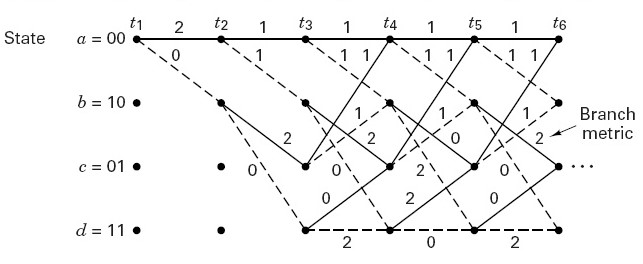
\includegraphics[scale=0.8]{encoder_trellis}
\caption{Diagram kratowy, dla enkodera o 3 bitowym rejestrze przesuwnym 
i dwóch sumatorach modulo-2 z wielomianami $g_1 = 111, g_2 = 101$ \protect\cite{Comm_Sklar}}
\label{fig:encoder_trellis}
\end{figure}


%\indent Dekoder viterbi 


%opisać rozpatrywany przypadek wykorzystania viterbiego
%do wyznaczania linii - arytkuły mazurek

%i chyba styka
\clearpage
\section{Implementacja w języku C++}
\indent Tworząc aplikację wykorzystującą algorytm Viterbiego do lokalizacji linii
na obrazie cyfrowym skorzystano z nowych funkcjonalności standardu C++11. 
Zdjęcia na, których szukano linii były wczytywane używając funkcji biblioteki
CImg. Reprezentowane przez obiekty \code{Cimg<T>}, dane pikseli zdjęcia były kopiowane do
dynamicznie zaalokowanych tablic jednowymiarowych obiektu \code{unique\_ptr}. Skorzystano z obiektu \code{unique\_ptr} w celu przechowywania wskaźnika do dynamicznie zaalokowanej pamięci, ze względu na funkcję automatycznego zwalniania zaalokowanych zasobów po wywołaniu destruktora \code{unique\_ptr}.  

%opis listinigu opencl_viterbi.cpp
\subsection{Wersja szeregowa}

%listing z viterbiLineDetect - nie pokazywac całego
\lstinputlisting[language={C++}, label={lst:viterbi_serial}, caption=Szeregowa implementacja algorytmu Viterbiego do wykrywania linii, linerange=224-297, firstnumber=224]{viterbi_source/Viterbi.cpp} 

%fragment inicjalizacja
\lstinputlisting[language={C++}, label={lst:viterbi_serial}, caption=Szeregowa implementacja algorytmu Viterbiego do wykrywania linii, linerange=224-240, firstnumber=224]{viterbi_source/Viterbi.cpp} 


%opisać wszystkie fragmenty z odniesieniem do schematu ogólnego algorytmu - shcemat z atykułów i wzory
\subsection{Wersja równoległa - C++11}
To jest podrozdział 2 rozdziału 2
\subsection{Wersja równoległa - OpenCL}
To jest podrozdział 3 rozdziału 2
\end{document}